\section{Referencia de la Clase Comp\-Articulo}
\label{classCompArticulo}\index{CompArticulo@{CompArticulo}}
Administra los datos de los componentes de un art\'{\i}culo.  


{\tt \#include $<$comparticulo.h$>$}

Diagrama de colaboraci\'{o}n para Comp\-Articulo:\begin{figure}[H]
\begin{center}
\leavevmode
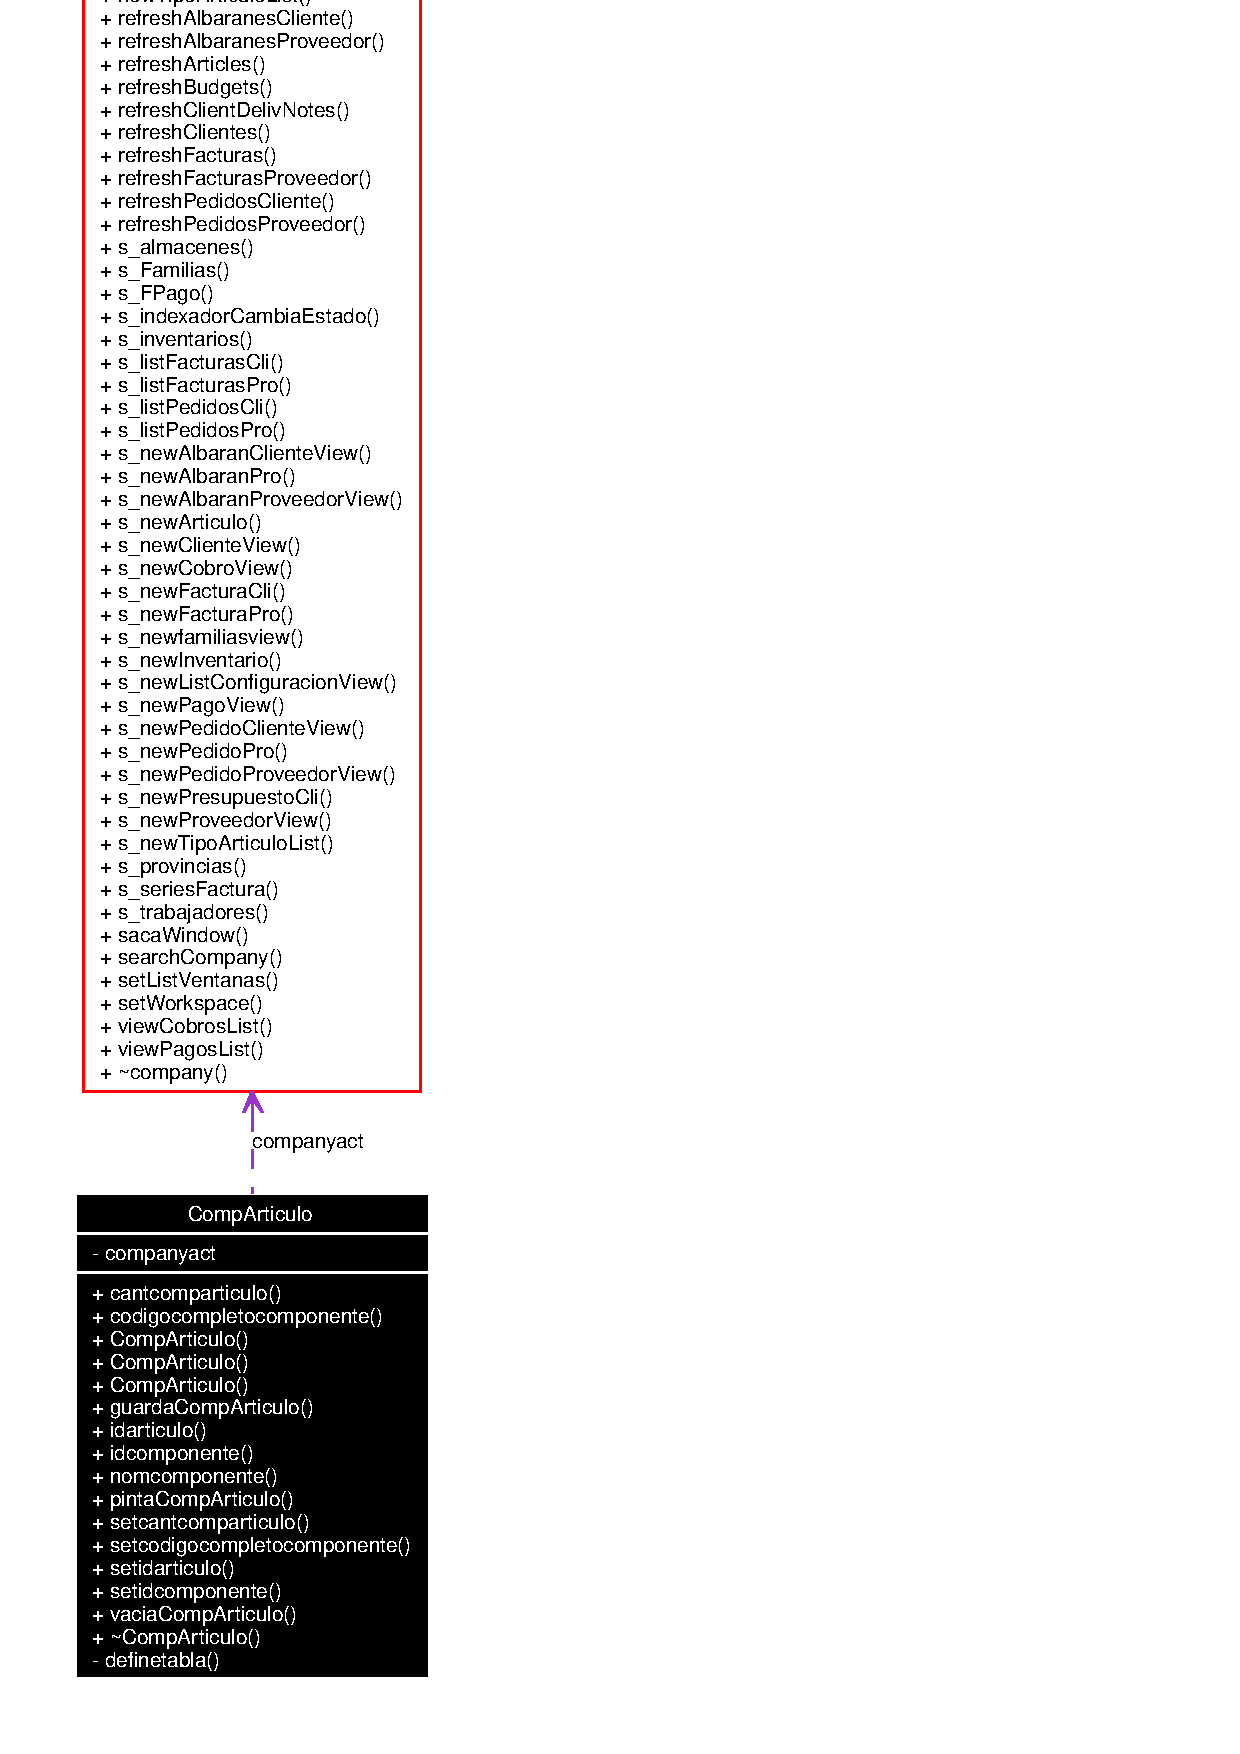
\includegraphics[width=103pt]{classCompArticulo__coll__graph}
\end{center}
\end{figure}
\subsection*{M\'{e}todos p\'{u}blicos}
\begin{CompactItemize}
\item 
QString {\bf cantcomparticulo} ()\label{classCompArticulo_a0}

\item 
QString {\bf codigocompletocomponente} ()\label{classCompArticulo_a1}

\item 
{\bf Comp\-Articulo} ({\bf company} $\ast$, QString, QString, QString, QString, QString)
\item 
{\bf Comp\-Articulo} ({\bf company} $\ast$, QString, QString)\label{classCompArticulo_a3}

\item 
{\bf Comp\-Articulo} ({\bf company} $\ast$)\label{classCompArticulo_a4}

\item 
void {\bf guarda\-Comp\-Articulo} ()
\item 
QString {\bf idarticulo} ()\label{classCompArticulo_a6}

\item 
QString {\bf idcomponente} ()\label{classCompArticulo_a7}

\item 
QString {\bf nomcomponente} ()\label{classCompArticulo_a8}

\item 
virtual void {\bf pinta\-Comp\-Articulo} ()\label{classCompArticulo_a9}

\item 
void {\bf setcantcomparticulo} (QString val)\label{classCompArticulo_a10}

\item 
void {\bf setcodigocompletocomponente} (QString)\label{classCompArticulo_a11}

\item 
void {\bf setidarticulo} (QString val)\label{classCompArticulo_a12}

\item 
void {\bf setidcomponente} (QString)\label{classCompArticulo_a13}

\item 
void {\bf vacia\-Comp\-Articulo} ()\label{classCompArticulo_a14}

\end{CompactItemize}


\subsection{Descripci\'{o}n detallada}
Administra los datos de los componentes de un art\'{\i}culo. 



\subsection{Documentaci\'{o}n del constructor y destructor}
\index{CompArticulo@{Comp\-Articulo}!CompArticulo@{CompArticulo}}
\index{CompArticulo@{CompArticulo}!CompArticulo@{Comp\-Articulo}}
\subsubsection{\setlength{\rightskip}{0pt plus 5cm}Comp\-Articulo::Comp\-Articulo ({\bf company} $\ast$, QString, QString, QString, QString, QString)}\label{classCompArticulo_a2}


La carga r\'{a}pida tiene un comportamiento poco restrictivo para aumentar la eficiencia. 

\subsection{Documentaci\'{o}n de las funciones miembro}
\index{CompArticulo@{Comp\-Articulo}!guardaCompArticulo@{guardaCompArticulo}}
\index{guardaCompArticulo@{guardaCompArticulo}!CompArticulo@{Comp\-Articulo}}
\subsubsection{\setlength{\rightskip}{0pt plus 5cm}void Comp\-Articulo::guarda\-Comp\-Articulo ()}\label{classCompArticulo_a5}


Segun esta la linea en la base de datos o no se hace una cosa u otra. 

La documentaci\'{o}n para esta clase fu\'{e} generada a partir de los siguientes archivos:\begin{CompactItemize}
\item 
comparticulo.h\item 
comparticulo.cpp\end{CompactItemize}
